\section{\texttt{Introduction}}
\begin{frame}{\textbf{Motivation}}

\begin{figure}
	\centering
	\begin{subfigure}[c]{0.3\textwidth}
		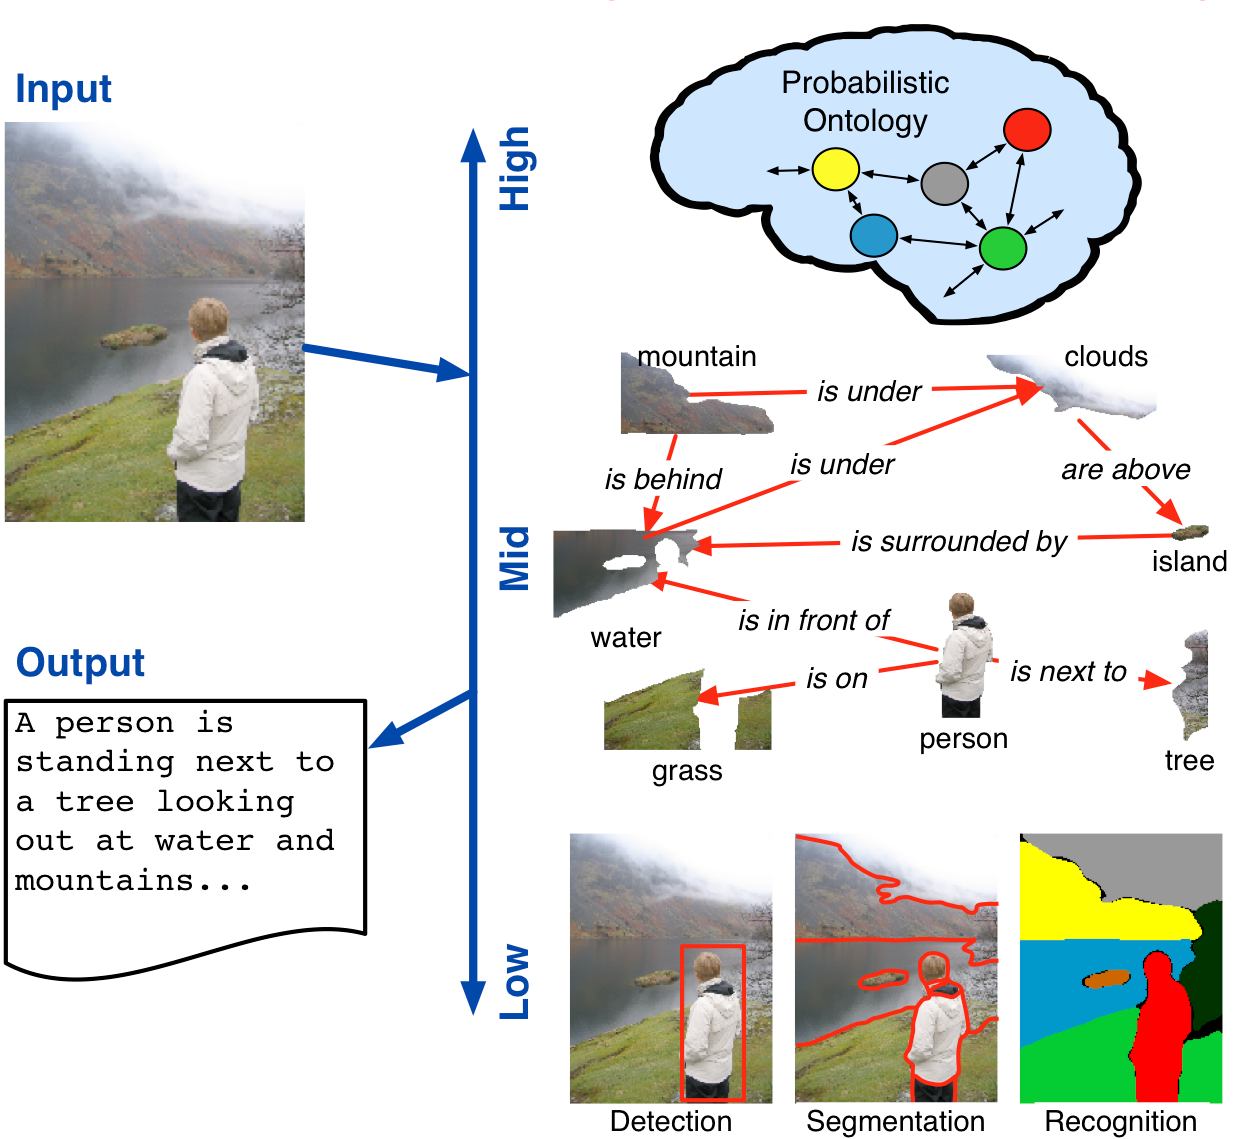
\includegraphics[width=\textwidth]{./img/motivation1.png} \footnotemark
    \end{subfigure}\hspace{3em}%
    \begin{subfigure}[c]{0.2\textwidth}
		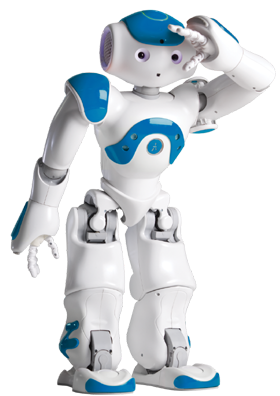
\includegraphics[width=\textwidth]{./img/motivation2.png} \footnotemark
    \end{subfigure}\hspace{3em}%
    \begin{subfigure}[c]{0.2\textwidth}
		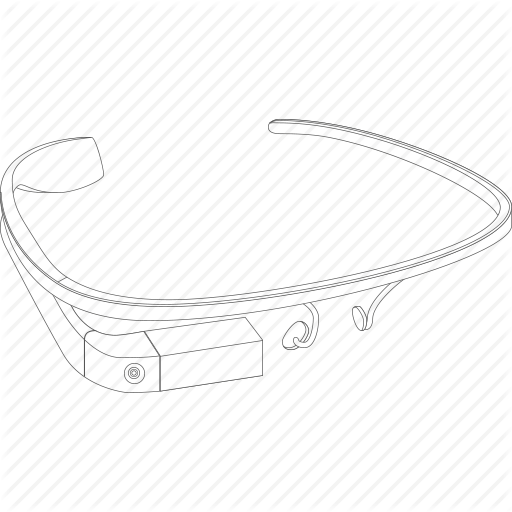
\includegraphics[width=\textwidth]{./img/motivation3.png} \footnotemark
    \end{subfigure}
\end{figure}
\footnotetext[1]{\tiny{\textbf{Generalized Image Understanding with Probabilistic Ontologies } (\url{http://www.cse.buffalo.edu/~jcorso/r/career}})}
\footnotetext[2]{\tiny{\textbf{Alderbaran robot nao } (\url{https://www.aldebaran.com/en/humanoid-robot/nao-robot})}}
\footnotetext[3]{\tiny{\textbf{Google glass } (\url{https://www.google.com/glass/start})}}
\end{frame}

\begin{frame}{\textbf{Objective}}
	\begin{columns}
		\begin{column}{0.55\textwidth}
		\begin{varblock}[\textwidth]{Problem}
			\begin{itemize}
				\item To detect and identify events in a given video segment.
			\end{itemize}
		\end{varblock}
		\begin{varblock}[\textwidth]{Challenges}
			\begin{itemize}
				\item Geometric and photometric variances
				\item Cluttered	 background 
				\item Complex camera motion
			\end{itemize}
		\end{varblock}
		\begin{varblock}[\textwidth]{Applications}
			\begin{itemize}
				\item Real time event recognition
				\item Automated video annotation
			\end{itemize}
		\end{varblock}
		\end{column}
		\begin{column}{0.38\textwidth}
			\centering
			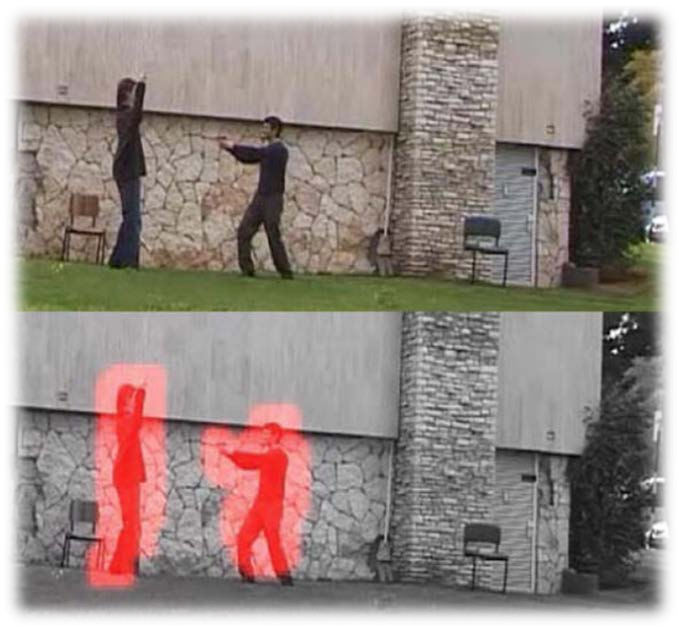
\includegraphics[width=\textwidth]{./img/example.png} \footnotemark
		\end{column}
	\end{columns}
\footnotetext[4]{\tiny{\textbf{UCSD Anomaly Detection Dataset } (\url{http://www.svcl.ucsd.edu/projects/anomaly})}}
\end{frame}


\begin{frame}{\textbf{Proposed Framework}}

\end{frame}